
%(BEGIN_QUESTION)
% Copyright 2011, Tony R. Kuphaldt, released under the Creative Commons Attribution License (v 1.0)
% This means you may do almost anything with this work of mine, so long as you give me proper credit

An Allen-Bradley PLC controls the starting and stopping of a conveyor belt, taking inputs from both hard-wired pushbutton switches as well as from an HMI panel connected to the PLC.  This particular system has a problem, though.  The conveyor starts, but the warning siren does not alert before start-up like it is supposed to.  The system worked perfectly just a few days ago.  A live-status view of the program seen while the conveyor is running reveals the following:

$$\includegraphics[width=15.5cm]{i03598x01.eps}$$

Based on the information gathered from this live-status view, what do you think is wrong with the system?  Explain your answer.

\underbar{file i03598}
%(END_QUESTION)





%(BEGIN_ANSWER)

{\it Half-credit for fault, half-credit for explanation why.}

\vskip 10pt

The problem is not with any input switches or with the HMI's signals to the PLC.  From all appearances, the PLC program is receiving the inputs it needs, and the program is functioning properly.  The problem most likely lies with the siren itself, the wiring to it, or the PLC's output channel sending power to the siren.

%(END_ANSWER)





%(BEGIN_NOTES)

{\bf This question is intended for exams only and not worksheets!}.

%(END_NOTES)


